\section{Assignments}\label{sec:assignments}

Assignments bezeichnen ein Feature von fulib.org, das sich mit dem Anlegen, Lösen und Bewerten von Hausaufgabenblättern sowie Online-Kursen beschäftigt.
Es handelt sich dabei um Modellierungsaufgaben in der Scenario-Sprache.
Diese können automatisch geprüft und manuell bewertet werden.
Dieser Abschnitt befasst sich zunächst mit dem Anlegen der Assignments aus Sicht des Kursleiters.
Daraufhin wird unter~\ref{subsec:solution} die Sicht der Studierenden bei der Lösung erläutert.
Auch des Vorgehen der Korrekteure zum Bewerten der Lösungen wird hier eläutert.
Zuletzt wird die Kurs-Funktion unter~\ref{subsec:courses} vorgestellt.

\subsection{Anlegen}\label{subsec:creation}

Das Anlegen von Assignments ist leicht im Footer unter Assignments \textrightarrow Create Assignment möglich.
Damit gelangt man auf das in Abbildung~\ref{fig:create-assignment} gezeigte Formular.

\begin{figure}
    \centering
    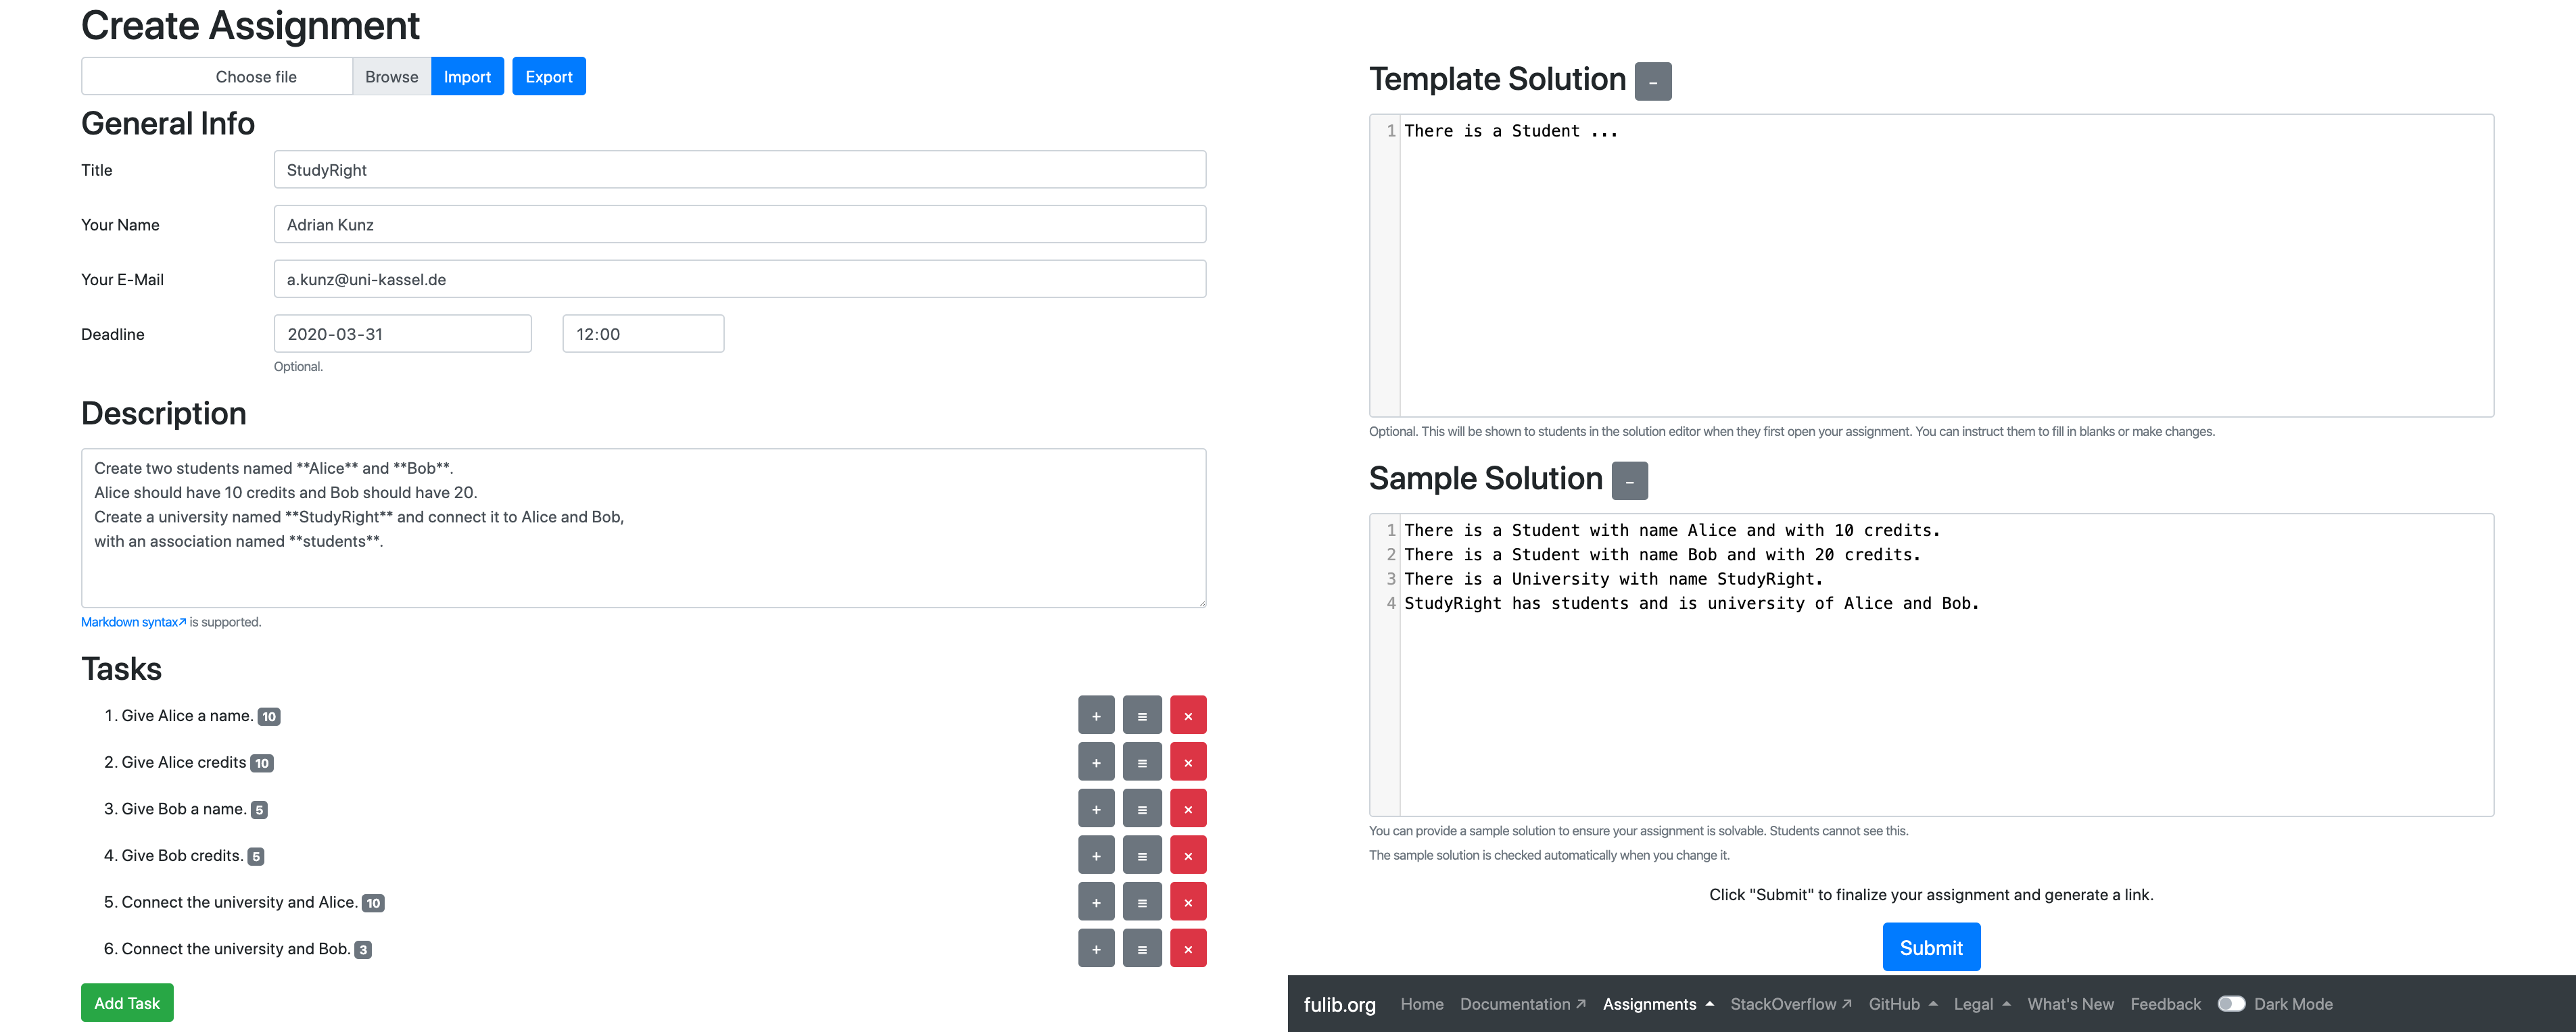
\includegraphics[width=0.5\textwidth]{chapter/fulib.org/img/create-assignment.png}
    \caption{Formular zum Anlegen von Assignments}
    \label{fig:create-assignment}
\end{figure}

Hier werden zunächst der Titel des Assignments sowie Name und E-Mail-Adresses zu Kursleiters eingetragen.
Ebenso muss eine Deadline angegeben werden.
Das mit ``Description'' bezeichnete Feld ist für die Aufgabenstellung vorgesehen.
Dabei wird Markdown-Syntax unterstützt, es können also Überschriften, Tabellen, Listen, Bilder etc.\ in jener verwendet werden.

Als nächstes werden die Teilaufgaben (Tasks) eingetragen.
Mit dem Button ``Add Task'' kann der Liste ein neuer Task hinzugefügt werden.
Jeder Task hat eine kurze Beschreibung und eine maximal erreichbare Punktzahl.
Der mit ``Verification'' bezeichnete Editor ist dafür vorgesehen, einen Teil eines Scenarios mit Expect-Sätzen einzutragen.
Ein Task wird später wie folgt automatisch bewertet:
Zunächst wird das hier eingetragene Teilscenario an die Lösung des Studierenden angehängt.
Das entstehende Scenario wird dann kompiliert und die entstandenen Tests werden ausgeführt.
Erzeugt dies einen Compilerfehler und schlägt der Test fehl, gilt die Teilaufgabe als nicht bestanden und wird mit null Punkten bewertet.
Andernfalls wird die maximal erreichbare Punktzahl vergeben.

Zur Übersichtlichkeit lassen sich die einzelnen Tasks mit dem ``+''- bzw.\ ``-''-Button ein- und ausklappen.
Mit der Schaltfläche rechts davon lassen sich Tasks durch Ziehen mit Maus bzw.\ Finger anordnen.
Der rote ``x''-Button löscht den Task aus der Liste.

Unter der Task-Liste befinden sich die Eingabefenster für die sogenannte ``Template Solution'' und die Musterlösung (Sample Solution).
Beide lassen sich mit den entsprechenden Buttons ein- und ausklappen, um das Formular übersichtlicher zu machen.
Gibt man eine Template Solution an, so wird diese den Studierenden als Lösung vorgegeben, wenn sie das Assignment öffnen.
Die Aufgabenstellung könnte dann beispielsweise sein, dass das vorgegebene Scenario angepasst oder vervollständigt wird.
Dafür könnten in der Template Solution z.B.\ Lücken mit ``\code{...}'' gelassen werden, die der Studierende ausfüllen soll.
Die Musterlösung ist zwar optional, sie erlaubt jedoch dem Ersteller, seine Aufgabenstellung auf Lösbarkeit zu prüfen.
Dadurch können Fehler in der Aufgabenstellung oder der Verifizierung frühzeutig erkannt werden.
Bei Änderung der Musterlösung wird diese automatisch geprüft.
In der Task-Liste werden dann diejenigen Tasks rot, deren Verifizierungscode fehlgeschlagen ist.
Dies deutet an, dass es ein Problem in der Musterlösung oder des Tasks gibt.

Sämtliche Änderungen am Formular werden sofort im Browser gespeichert.
Dadurch ist Datenverlust beim Verlassen der Seite oder bei Ausfall der Internetverbindung ausgeschlossen.
Dennoch gibt es die Möglichkeit, den Entwurf des Assignments als Datei auf der Festplatte zu speichern.
Dies ist mit dem ``Export''-Button möglich.
Später kann diese Datei dann wieder in das Formular übernommen werden.
Dafür muss diese im Feld neben dem ``Import''-Button ausgewählt werden und anschließend auf diesen geklickt werden.
Die Import/Export-Funktion erlaubt ferner, ein Assignment für die spätere Bearbeitung zu speichern und ein Neues zu erstellen.
Heruntergeladene Datein können weiterhin über E-Mail oder Filesharing an andere weitergegeben werden,
die das Assignment dann importieren und prüfen oder verändern können.

Um ein fertiges Assignment zu veröffentlich, genügt ein Klick auf den ``Submit''-Button.
Dieser bewirkt, dass das ausgefüllte Formular an den Server gesendet wird, der das erstellte Assignment speichert und einen Link generiert.
Abbildung~\ref{fig:create-assignment-success} zeigt das Fenster, das sich daraufhin öffnet und diesen Link zeigt.

\begin{figure}
    \centering
    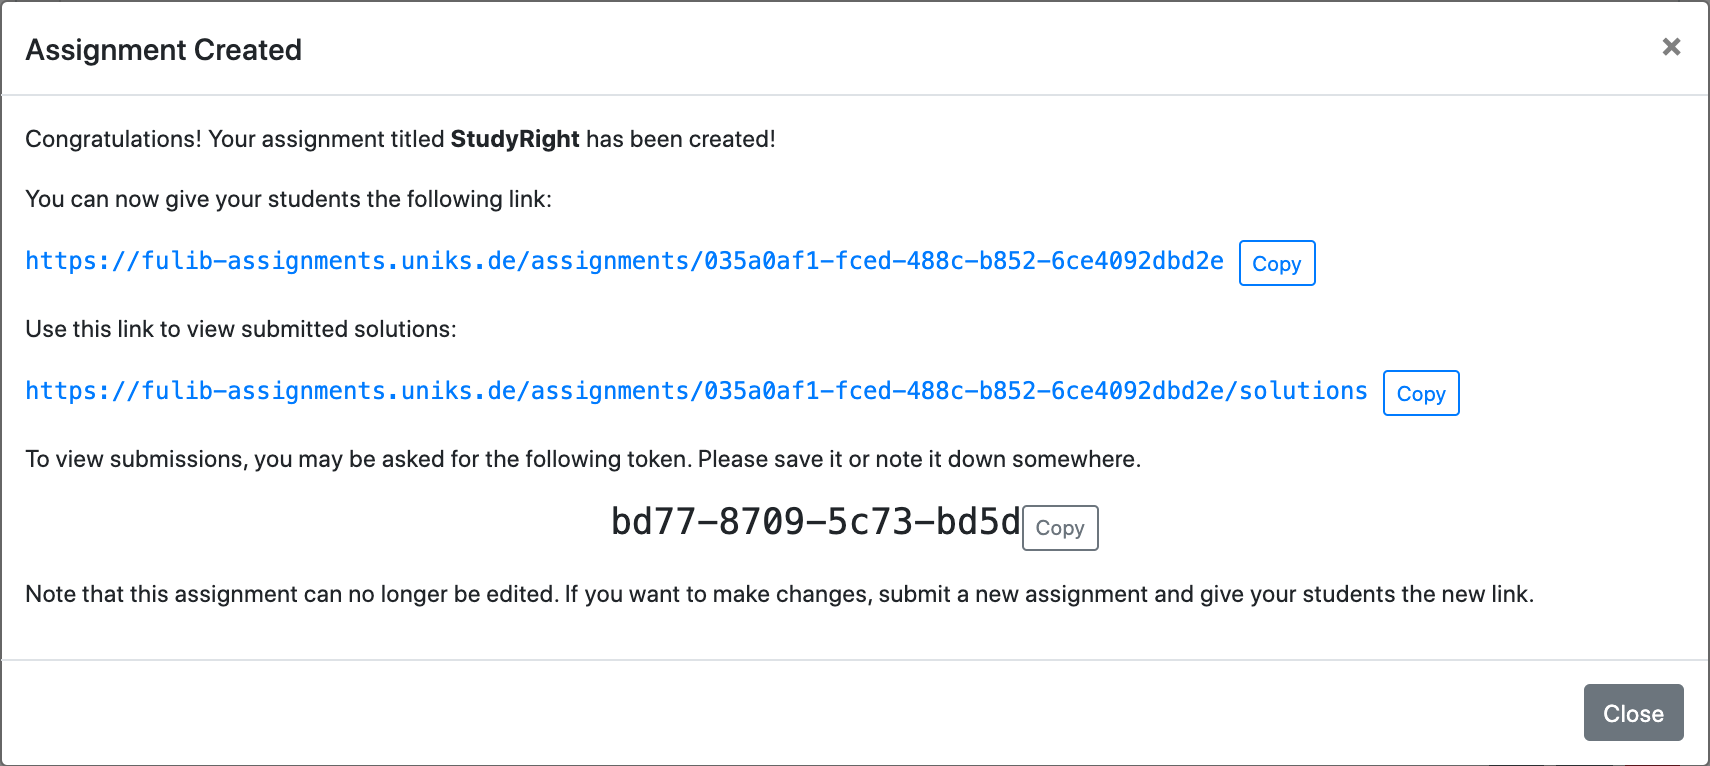
\includegraphics[width=\textwidth]{chapter/fulib.org/img/create-assignment-success.png}
    \caption{Fenster nach Anlegen eines Assignments}
    \label{fig:create-assignment-success}
\end{figure}

Der erste Link ist dafür vorgesehen, ihn an die Studierenden weiterzuleiten.
Öffnen sie diesen, zeigt sich die Seite, in der sie ihre Lösung des Assignments erstellen und abgeben können.
Dieser Vorgang ist Thema des nächsten Unterabschnitts.
Der zweite Link ist für den Kursleiter und die Korrekteure, da darunter eine Liste aller abgegeben Lösungen zu finden ist.
Um darauf zugreifen zu können, wird das gezeigte Token benötigt.
Dieses muss vom Kursleiter an die Korrekteure weitergeleitet werden.
Ohne dieses Token-System könnten Studierende die Lösungen von Anderen einsehen und übernehmen.

Assignments sind nach dem Einreichen nicht mehr veränderbar.
Dies ist gewünscht, da das Verändern von Assignments, die schon von Studierenden bearbeitet wurden, für diese nachteilhaft ist.
Wird im Nachhinein ein Fehler in der Aufgabenstellung erkannt, kann das gleiche Assignment erneut eingereicht werden.
Dabei werden neue Links und Token generiert, die wieder entsprechend geteilt werden müssen.

\subsection{Lösen}\label{subsec:solution}

\todo{
Shareable-Link-Ansatz.
Automatische Überprüfung.
Unveränderbar-Ansatz und Versionshistorie.
}

\subsection{Korrigieren}\label{subsec:correcting}

\todo{
Berechtigungssystem.
Workflow.
Kommentare.
Anpassbare Bepunktung.
}

\subsection{Kurse}\label{subsec:courses}

\todo{
Anlegen,
Seitenleiste,
FulibScenarios-Kurs
}
